\section{Norwegian dialects}
\label{sec:dialects-dialectology}

The Norwegian dialect landscape is generally divided into four dialect groups: East Norwegian, West Norwegian, Trønder,%
\footnote{Trønder dialects are mostly spoken in Trøndelag county in central Norway.}
and North Norwegian 
(\citeauthor{jahr1990dialekter}, \citeyear{jahr1990dialekter}, p.~10; \citeauthor{maehlum2012dialektlandskapet}, \citeyear{maehlum2012dialektlandskapet}, pp.~32--42; \citeauthor{bardhdal1997nordiska}, \citeyear{bardhdal1997nordiska}, pp.~263--264; \citeauthor{hanssen2010dialekter}, p.~118).
\autoref{fig:norway-map} shows the geographic areas in which the different dialect groups are spoken.

\begin{figure}[ht]
    \centering
    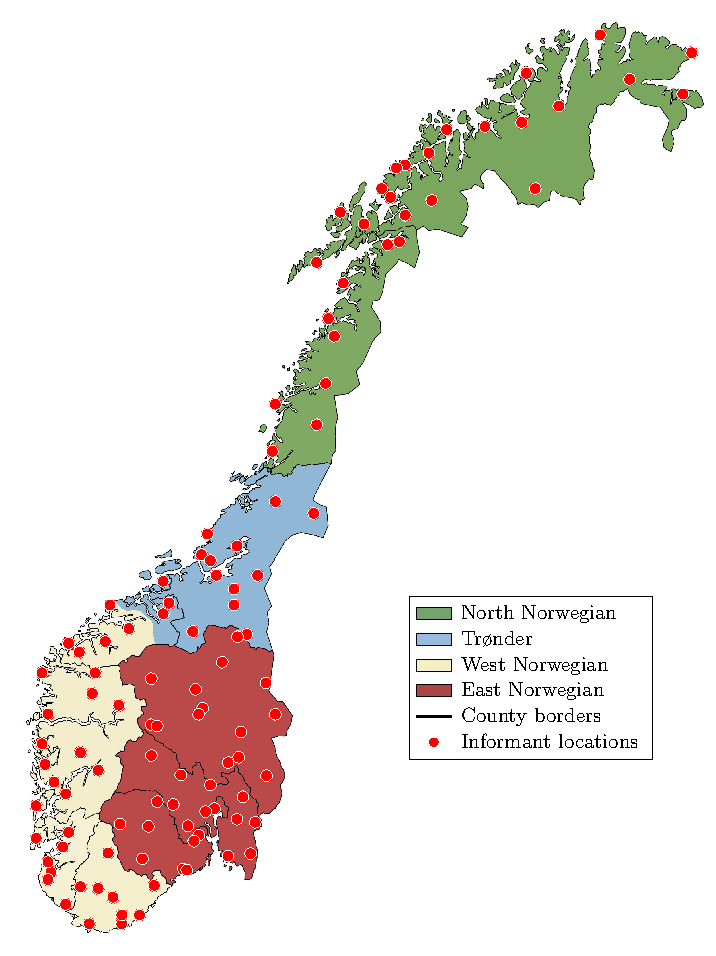
\includegraphics[width=\textwidth]{figures/3-dialects/dialect-map.pdf}
    \caption
    [Dialect areas in Norway and ScanDiaSyn informant locations]
    {Dialect areas in Norway and ScanDiaSyn informant locations.
    The division into dialect areas follows the one by \citet[p.~178]{maehlum2012dialektlandskapet}.}
    \label{fig:norway-map}
\end{figure}


This division is based on linguistic properties that I later explain in \autoref{sec:dialects-results-lingmajor}.
To some degree, such linguistic boundaries also match certain natural borders. For instance, the linguistic border between the West and East Norwegian dialect groups largely coincides with a mountain range separating the two geographic areas \cite[p.~104]{sandoey1991dialektkunnskap}.

The split into dialect groups is not entirely clear-cut, but complicated by several factors.
There is ample variation within each group, and there exist dialects that act as transition zones between the more characteristic varieties of different dialect groups \cite[p.~29]{maehlum2012dialektlandskapet}. 
Furthermore, individual regions within Northern Norway are influenced by linguistic contact in ways that do not apply to the majority of other Norwegian dialects (contact with Sámi languages and with dialects spoken by East Norwegian settlers) (\citeauthor{maehlum2012dialektlandskapet}, \citeyear{maehlum2012dialektlandskapet}, pp.~116; \citeauthor{jahr1990dialekter}, \citeyear{jahr1990dialekter}, pp.~180, 182).

% The inner part of the (former) county Troms experienced an influx of South East Norwegian settlers in the late 18th and early-to-mid 19th century \cite[p.~115]{maehlum2012dialektlandskapet}.
% To this day, the dialects spoken in this area contain dialect traits from both East and North Norwegian, to different degrees (\citeauthor{maehlum2012dialektlandskapet}, \citeyear{maehlum2012dialektlandskapet}, pp.~116; \citeauthor{jahr1990dialekter}, \citeyear{jahr1990dialekter}, pp.~180, 182).

\FloatBarrier